\documentclass{jarticle}
\usepackage{amsmath,amssymb}
\usepackage{amsmath}
\usepackage[dvipdfmx]{graphicx}
\usepackage{here}
\usepackage{pifont}
\usepackage[left=2cm, right=2cm]{geometry}
\setcounter{MaxMatrixCols}{20}
\begin{document}
\title{BdGハミルトニアン}
\author{金沢彰太郎}
\maketitle

\tableofcontents
\newpage
\section{導入}
BdGにおける分散関係と状態密度を求めることを目標にする。
BdGハミルトニアンは以下の式で表される。
\begin{align}
\mathcal{H}=\int\vec{\Psi}^\dagger(x,y)\hat{H}\vec{\Psi}(x,y)dr
\end{align}
ここで
\begin{align}
\int{dr}=\int{dxdy}
\end{align}
である。
\begin{align}
\vec{\Psi}=\begin{bmatrix}
\psi_{\uparrow} \\
\psi_{\downarrow} \\
\psi_{\uparrow}^\dagger \\
\psi_{\downarrow}^\dagger
\end{bmatrix}
\end{align}
ハミルトン演算子は次のようである。
\begin{align}
\hat{H}=
\begin{pmatrix}
\hat{h}(r) & \hat{\Delta}(r) \\
-\hat{\Delta}^{*}(r) & -\hat{h}^{*}(r)
\end{pmatrix}
\end{align}
ただし
\begin{align}
\hat{H}\in\mathbb{C}^{4\times 4}
\end{align}
\begin{align}
\hat{\Delta}(r),\hat{h}(r)\in\mathbb{C}^{2\times 2}
\end{align}
\begin{align}
\hat{h}=
\begin{bmatrix}
-\dfrac{\hbar^2}{2m}\nabla^2-\mu_F
\end{bmatrix}
\hat{\sigma}_0
\end{align}
\begin{flushright}
	$\hat{\sigma}_0$: 単位行列
\end{flushright}
\begin{align}
\nabla^2=\partial_x^2+\partial_y^2	
\end{align}
である。
$\hat{\Delta}(r)$の中身を次の三通りで考えていく。
\begin{align}
\hat{\Delta}(r)=
\begin{cases}
$\rm(\hspace{.18em}i\hspace{.18em})\quad$\Delta_0(i\sigma_2)
& \mbox{$s$-wave}
\vspace*{1em}\\
$\rm(\hspace{.18em}ii\hspace{.18em})$\quad\Delta_0\dfrac{i\partial x}{k_F}\hat\sigma_1
& \mbox{$p_x$-wave}
\vspace*{1em}\\
$\rm(\hspace{.18em}iii\hspace{.18em})$\quad\Delta_0\dfrac{1}{k_F}(\partial x+i\partial y)\hat\sigma_1\
& \mbox{$p_x+ip_y$-wave}
\end{cases}
\label{delta}
\end{align}
\begin{figure}[H]
	\centering
	%	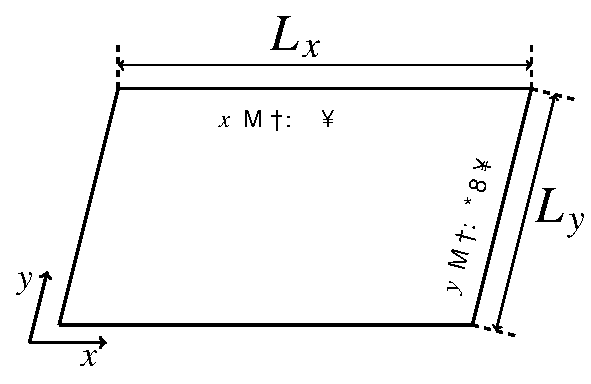
\includegraphics[scale=1]{./figure1.pdf}
	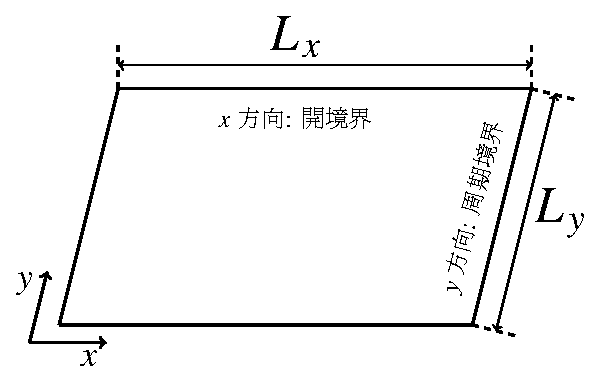
\includegraphics[scale=1]{../../14/KS/figure_fix.pdf}
	\caption{考える系}
	\label{system}
\end{figure}
図\ref{system}の系を考える。$y$方向には境界条件が課されている。
\begin{align}
\vec{\Psi}=\dfrac{1}{\sqrt{L_y}}\displaystyle\sum_{k_y}\vec{\Psi}_{k_y}(x)e^{ik_yy}
\end{align}
%式\eqref{delta}
1.(i)の$\hat{\Delta}$を使う\\		                                               	%itemizeやenumearteという箇条書きする環境があるので調べてみましょう
\ding{"AB} $H$をフーリエ変換しましょう!$y$を波数に変換して一旦固定して$x$の関数として考えます。
\\ ヒント: (1)に(2)を代入しましょう。\\
\ding{"AD}離散化しましょう\\
\begin{align}
\mathcal{H}\rightarrow \tilde{\mathcal{H}}
\end{align}
\begin{align}
\tilde{\mathcal{H}}=\vec{\Psi^{\dagger}}\hat{H}\vec{\Psi}	
\end{align}
\begin{align}
\vec{\Psi}=\begin{bmatrix}
\psi_{1\uparrow} \\
\psi_{1\downarrow} \\
\psi_{1\uparrow}^\dagger \\
\psi_{1\downarrow}^\dagger\\
\psi_{2\uparrow} \\
\psi_{2\downarrow} \\
\vdots
\end{bmatrix}
\end{align}
\begin{align}
\tilde{H}=
\begin{pmatrix}
\hat{H} &  &  &  \\
& \hat{H} &  &  \\
&  & \hat{H} &  \\
&  &  & \ddots
\end{pmatrix}
\end{align}
\begin{align}
\dfrac{\hbar^2}{2m}=t
\end{align}
とする。\\
\ding{"AE}差分近似しましょう\\
\begin{align}
\partial_x \psi_i\rightarrow?\\
\partial^2_x \psi_i\rightarrow?\\
\end{align}
刻み幅は$1$\\
\ding{"AF}$\tilde{H}$を対角化しましょう。数値計算\\
2(ii)の$\hat{\Delta}$を使う\\
3(iii)の$\hat{\Delta}$を使う\\

\section{計算・結果}
\subsection{1の場合}
	\begin{align}
	\mathcal{H}=\int\vec{\Psi}^\dagger(x,y)\hat{H}\vec{\Psi}(x,y)dr
	\end{align}
	に
	\begin{align}
	\vec{\Psi}=\dfrac{1}{\sqrt{L_y}}\displaystyle\sum_{k_y}\vec{\Psi}_{k_y}(x)e^{ik_yy}
	\end{align}
	を代入していく。
	ここで
	\begin{align}
	\vec{\Psi}^\dagger=\dfrac{1}{\sqrt{L_y}}\displaystyle\sum_{k_y^{'}}\vec{\Psi}^\dagger_{k_y^{'}}(x)e^{-ik_y^{'}y}
	\end{align}
	であるから
	\begin{align}
	\mathcal{H}&=\int\dfrac{1}{\sqrt{L_y}}\displaystyle\sum_{k_y^{'}}\vec{\Psi}^\dagger_{k_y^{'}}(x)e^{-ik_y^{'}y}\hat{H}\dfrac{1}{\sqrt{L_y}}\displaystyle\sum_{k_y}\vec{\Psi}_{k_y}(x)e^{ik_yy}(x,y)dr\\&=\dfrac{1}{L_y}\underline{\int\displaystyle\sum_{k_y^{'}}\vec{\Psi}^\dagger_{k_y^{'}}(x)e^{-ik_y^{'}y}\hat{H}\displaystyle\sum_{k_y}\vec{\Psi}_{k_y}(x)e^{ik_yy}(x,y)dr}\\
	\label{star}
	\end{align}
	\\となる。下線部について計算していく。
	\begin{align}
	\tilde{H}&=
	\begin{pmatrix}
	\hat{h}(r) & \hat{\Delta}(r) \\
	-\hat{\Delta}^{*}(r) & -\hat{h}^{*}(r)
	\end{pmatrix}
	\\&=
	\begin{pmatrix}
	(-\dfrac{\hbar^2}{2m}\nabla^2-\mu_F)\hat{\sigma}_0 & \Delta_0(i\sigma_2) \\
	-\Delta^{*}_0(i\sigma^{*}_2) & (\dfrac{\hbar^2}{2m}\nabla^2+\mu_F)\hat{\sigma}^{*}_0		
	\end{pmatrix}
	\end{align}
	ここで
	$\hat\sigma_0$、$\hat\sigma_2$はパウリ行列であり、
	\begin{align}
	\hat{\sigma_0}=
	\begin{pmatrix}
	1 & 0 \\
	0 & 1
	\end{pmatrix},
	\hat{\sigma_2}=
	\begin{pmatrix}
	0 & -i \\
	i & 0
	\end{pmatrix}
	\end{align}
	である。
	\begin{align}
	\tilde{H}&=
	\begin{pmatrix}
	(-\dfrac{\hbar^2}{2m}\nabla^2-\mu_F)\begin{pmatrix}
	1 & 0 \\
	0 & 1
	\end{pmatrix} & \Delta_0i \begin{pmatrix}
	0 & -i \\
	i & 0
	\end{pmatrix} \\
	-\Delta^{*}_0\begin{pmatrix}
	0 & -1 \\
	1& 0
	\end{pmatrix} & (\dfrac{\hbar^2}{2m}\nabla^2+\mu_F)\begin{pmatrix}
	1 & 0 \\
	0 & 1
	\end{pmatrix}
	\end{pmatrix}
	\\&=\begin{pmatrix}
	\xi & 0 & 0 & \Delta_0 \\ 
	0 & \xi & -\Delta_0 & 0 \\ 
	0 & -\Delta^{*}_0 & -\xi & 0 \\ 
	\Delta^{*}_0 & 0 & 0 & -\xi
	\end{pmatrix} 
	\end{align}
	ここで
	\begin{align}
	-\dfrac{\hbar^2}{2m}\nabla^2-\mu_F=\xi
	\end{align}
	とした。式\eqref{star}の下線部は\\		
	\begin{align}
	\begin{split}
	\int&\displaystyle\sum_{k_y}\sum_{k_y^{'}}\begin{pmatrix}
	\psi_{\uparrow}^{\dagger}e^{-ik_y^{'}y} & \psi_{\downarrow}^{\dagger}e^{-ik_y^{'}y} & \psi_{\uparrow}e^{-ik_y^{'}y} & \psi_{\downarrow}e^{-ik_y^{'}y}
	\end{pmatrix}
	\begin{pmatrix}
	\xi & 0 & 0 & \Delta_0 \\ 
	0 & \xi & -\Delta_0 & 0 \\ 
	0 & -\Delta^{*}_0 & -\xi & 0 \\ 
	\Delta^{*}_0 & 0 & 0 & -\xi
	\end{pmatrix}
	\displaystyle\begin{bmatrix}
	\psi_{\uparrow}e^{ik_yy} \\
	\psi_{\downarrow}e^{ik_yy} \\
	\psi_{\uparrow}^{\dagger} e^{ik_yy}\\
	\psi_{\downarrow}^{\dagger}e^{ik_yy}
	\end{bmatrix}dxdy
	\\=\int\displaystyle\sum_{k_y}&\sum_{k_y^{'}}\psi_{\uparrow}^{\dagger}e^{-ik_y^{'}y}(\xi\psi_{\uparrow}e^{ik_yy}+\Delta^{*}_0\psi_{\downarrow}^{\dagger}e^{ik_yy})\\&
	+\psi_{\downarrow}^{\dagger}e^{-ik_y^{'}y}(\xi\psi_{\downarrow}e^{ik_yy}-\Delta^{*}_0\psi_{\uparrow}^{\dagger}e^{ik_yy})\\&
	+\psi_{\uparrow}e^{-ik_y^{'}y}(-\Delta_0\psi_{\downarrow}^{*}e^{ik_yy}-\nabla^{'}\psi_{\uparrow}^{*}e^{ik_yy})\\&
	+\psi_{\downarrow}e^{-ik_y^{'}y}(\Delta_0\psi_{\uparrow}^{*}e^{ik_yy}-\nabla^{'}\psi_{\downarrow}^{*}e^{ik_yy})
	\end{split}	                                                          
	\end{align}
	第一項について
	\begin{align}
	&\int\displaystyle\sum_{k_y}\sum_{k_y^{'}}\psi_{\uparrow}^{\dagger}e^{-ik_y^{'}y}(\xi\psi_{\uparrow}e^{ik_yy}+\Delta^{*}_0\psi_{\downarrow}^{\dagger}e^{ik_yy})dxdy\\
	&=\int\displaystyle\sum_{k_y}\sum_{k_y^{'}}\psi_{\uparrow}^{\dagger}e^{-ik_y^{'}y}[(-\dfrac{\hbar^2}{2m}\nabla^2-\mu_F)\psi_{\uparrow}e^{ik_yy}+\Delta^{*}_0\psi_{\downarrow}^{\dagger}e^{ik_yy}]dxdy\\
	\end{align}
	$\nabla^2$の計算を行う。
	\begin{align}
	\nabla^{2}\psi_{\uparrow}e^{ik_yy}&=(\partial_x^2+\partial_y^2)\psi_{\uparrow}e^{ik_yy}\\
	&=\partial_x^2\psi_{\uparrow}e^{ik_yy}+\partial_y^2\psi_{\uparrow}e^{ik_yy}\\
	&=e^{ik_yy}\partial_x^2\psi_{\uparrow}-k^{2}_ye^{ik_yy}\psi_{\uparrow}
	\end{align}
	であるから
	\begin{align}
	\int\displaystyle\sum_{k_y}\sum_{k_y^{'}}\psi_{\uparrow}^{\dagger}e^{-ik_y^{'}y}\Big[\big\{-\dfrac{\hbar^2}{2m}(\dfrac{\partial^{2}}{\partial x^2}-k^{2}_y)-\mu_F\big\}\psi_{\uparrow}e^{ik_yy}+\Delta^{*}_0\psi_{\downarrow}^{\dagger}e^{ik_yy}\Big]dxdy
	\end{align}
	ここで
	\begin{align}
	\int\displaystyle\sum_{k_y}\sum_{k_y^{'}}\psi^{\dagger}e^{-ik_y^{'}y}e^{ik_yy}{\psi}dy=L_y\sum_{k_y}\psi^{\dagger}\psi
	\end{align}
	を用いて
	\begin{align}
	\int\displaystyle\sum_{k_y}L_y\Big[\psi_{\uparrow}^{\dagger}\big\{-\dfrac{\hbar^2}{2m}(\dfrac{\partial^{2}}{\partial x^2}-k^{2}_y)-\mu_F\big\}\psi_{\uparrow}+\psi_{\uparrow}^{\dagger}\Delta^{*}_0\psi_{\downarrow}^{\dagger}\Big]dx
	\end{align}
	従って$\mathcal{H}$は
	\begin{align}
	\mathcal{H}=\int\displaystyle\sum_{k_y}&\Big[\psi_{\uparrow}^{\dagger}\big\{-\dfrac{\hbar^2}{2m}(\dfrac{\partial^{2}}{\partial x^2}-k^{2}_y)-\mu_F\big\}\psi_{\uparrow}+\psi_{\uparrow}^{\dagger}\Delta^{*}_0\psi_{\downarrow}^{\dagger}\\
	&+\psi_{\downarrow}^{\dagger}\big\{-\dfrac{\hbar^2}{2m}(\dfrac{\partial^{2}}{\partial x^2}-k^{2}_y)-\mu_F\big\}\psi_{\downarrow}-\psi_{\downarrow}^{\dagger}\Delta^{*}_0\psi_{\uparrow}^{\dagger}\\
	&-\psi_{\uparrow}^{\dagger}\big\{-\dfrac{\hbar^2}{2m}(\dfrac{\partial^{2}}{\partial x^2}-k^{2}_y)-\mu_F\big\}\psi_{\uparrow}^{\dagger}-\psi_{\uparrow}\Delta_0\psi_{\downarrow}^{\dagger}\\
	&-\psi_{\downarrow}\big\{-\dfrac{\hbar^2}{2m}(\dfrac{\partial^{2}}{\partial x^2}-k^{2}_y)-\mu_F\big\}\psi_{\downarrow}^{\dagger}+\psi_{\downarrow}\Delta_0\psi_{\uparrow}\Big]dx
	\end{align}
	積分$\int$を和記号$\sum$にして$x$を離散化していく。刻み幅を$1$とすると
	\begin{align}
	\int dx\rightarrow\sum_{i=1}^{L_y+1}\Delta x=\sum_{i=1}^{L_y+1}
	\end{align}
	となる。また波動関数を
	\begin{align}
	\psi(x_i)\rightarrow\psi_i		
	\end{align}
	と離散化する。すると$\mathcal{H}$は
	\begin{align}
	\mathcal{H}&=\sum_{i=1}^{L_y+1}\displaystyle\sum_{k_y}\Big[\psi_{i\uparrow}^{\dagger}\big\{-\dfrac{\hbar^2}{2m}(\dfrac{\partial^{2}}{\partial x^2}-k^{2}_y)-\mu_F\big\}\psi_{i\uparrow}+\psi_{i\uparrow}^{\dagger}\Delta^{*}_0\psi_{i\downarrow}^{\dagger}\cdots\Big]dx\\
	&=\sum_{i=1}^{L_y+1}\displaystyle\sum_{k_y}\Big[-\dfrac{\hbar^2}{2m}(\psi_{i\uparrow}^{\dagger}\dfrac{\partial^{2}}{\partial x^2}\psi_{i\uparrow})+(\dfrac{\hbar^2k^{2}_y}{2m}-\mu_F)\psi_{i\uparrow}^{\dagger}\psi_{i\uparrow}+\psi_{i\uparrow}^{\dagger}\Delta^{*}_0\psi_{i\downarrow}^{\dagger}\cdots\Big]dx
	\end{align}
	ここで$\dfrac{\partial^{2}}{\partial x^2}\psi_{i\uparrow}$を差分近似する。関数を次のように近似する。
	\begin{align}
	\dfrac{\partial^{2}}{\partial x^2}f(x)=\dfrac{f(x+h)-2f(x)+f(x-h)}{h^2}
	\end{align}
	刻み幅$1$で$x$を$i$で書けば
	\begin{align}
	\dfrac{\partial^{2}}{\partial x^2}f(i)=f(i+1)-2f(i)+f(i-1)
	\end{align}
	これより$\mathcal{H}$は
	\begin{align}
	\mathcal{H}
	=\sum_{i=1}^{L_y+1}\displaystyle\sum_{k_y}\Big[\big\{\dfrac{\hbar^2}{2m}(k_y^2+2)-\mu\big\}\psi_{i\uparrow}^{\dagger}\psi_{i\uparrow}-\Lambda\psi_{i\uparrow}^{\dagger}\psi_{i+1\uparrow}-\Lambda\psi_{i\uparrow}^{\dagger}\psi_{i-1\uparrow}+\psi_{i\uparrow}^{\dagger}\Delta^{*}_0\psi_{i\downarrow}^{\dagger}\cdots\Big]dx
	\end{align}
	ここで
	\begin{align}
	\Lambda=\dfrac{\hbar^2}{2m}
	\end{align}
	とおいた。
	\begin{align}
	\varepsilon_{k_y}=\dfrac{\hbar^2}{2m}(k_y^2+2)-\mu
	\end{align}
	とすると全体の$\mathcal{H}$は行列で書けて三つ分書くと
	\begin{align}
	\mathcal{H}=
	\begin{bmatrix}
	\psi_{1\uparrow}^\dagger \\ 
	\psi_{1\downarrow}^\dagger \\ 
	\psi_{1\uparrow} \\ 
	\psi_{1\downarrow} \\ 
	\psi_{2\uparrow}^\dagger \\ 
	\psi_{2\downarrow}^\dagger \\ 
	\psi_{2\uparrow} \\ 
	\psi_{2\downarrow} \\ 
	\psi_{3\uparrow}^\dagger \\ 
	\psi_{3\downarrow}^\dagger \\ 
	\psi_{3\uparrow} \\ 
	\psi_{3\downarrow}
	\end{bmatrix} 
	^T
	\begin{bmatrix}
	\varepsilon_{k_y} & 0 & 0 & \Delta_0 & -\Lambda & 0 & 0 & 0 & 0 & 0 & 0 & 0 \\ 
	0 & \varepsilon_{k_y} & -\Delta_0 & 0 & 0 & -\Lambda & 0 & 0 & 0 & 0 & 0 & 0 \\ 
	0 & -\Delta_0^{*} & -\varepsilon_{k_y} & 0 & 0 & 0 & \Lambda & 0 & 0 & 0 & 0 & 0 \\ 
	\Delta_0^{*} & 0 & 0 & -\varepsilon_{k_y} & 0 & 0 & 0 & \Lambda & 0 & 0 & 0 & 0 \\ 
	-\Lambda & 0 & 0 & 0 & \varepsilon_{k_y} & 0 & 0 & \Delta_0 & -\Lambda & 0 & 0 & 0 \\ 
	0 & -\Lambda & 0 & 0 & 0 & \varepsilon_{k_y} & -\Delta_0 & 0 & 0 & -\Lambda & 0 & 0 \\ 
	0 & 0 & \Lambda & 0 & 0 & -\Delta_0^{*} & -\varepsilon_{k_y} & 0 & 0 & 0 & \Lambda & 0 \\ 
	0 & 0 & 0 & \Lambda & \Delta_0^{*} & 0 & 0 & -\varepsilon_{k_y} & 0 & 0 & 0 & \Lambda \\ 
	0 & 0 & 0 & 0 & -\Lambda & 0 & 0 & 0 & \varepsilon_{k_y} & 0 & 0 & \Delta_0 \\ 
	0 & 0 & 0 & 0 & 0 & -\Lambda & 0 & 0 & 0 & \varepsilon_{k_y} & -\Delta_0 & 0 \\ 
	0 & 0 & 0 & 0 & 0 & 0 & \Lambda & 0 & 0 & -\Delta_0^{*} & \varepsilon_{k_y} & 0 \\ 
	0 & 0 & 0 & 0 & 0 & 0 & 0 & \Lambda & \Delta_0^{*} & 0 & 0 & -\varepsilon_{k_y}
	\end{bmatrix} 
	\begin{bmatrix}
	\psi_{1\uparrow} \\ 
	\psi_{1\downarrow} \\ 
	\psi_{1\uparrow}^\dagger \\ 
	\psi_{1\downarrow}^\dagger \\ 
	\psi_{2\uparrow} \\ 
	\psi_{2\downarrow} \\ 
	\psi_{2\uparrow}^\dagger \\ 
	\psi_{2\downarrow}^\dagger \\ 
	\psi_{3\uparrow} \\ 
	\psi_{3\downarrow} \\ 
	\psi_{3\uparrow}^\dagger \\ 
	\psi_{3\downarrow}^\dagger
	\end{bmatrix} 
	\end{align}
	となる。ここから$\mathcal{H}$を数値計算で対角化していく。
$\mathcal{H}$を数値計算で対角化していく。	この時$\mu=3.5, \Lambda=1.0, \Delta=1.0$	とした。
$N=100$、$k_y$を横軸として変化させて縦軸に固有値をプロットし分散関係を描いた。結果は以下のようになった。\\		
\begin{figure}[H]
	\centering
	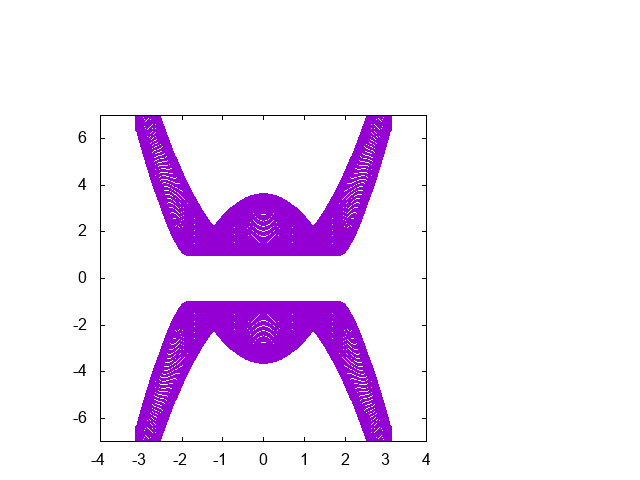
\includegraphics{../../16/KS/16-1/graph/data.png}			%もし余力がありましたら, 軸にラベルを(縦軸にエネルギー,横軸にky)をつけてみましょう
	\caption{分散関係}
\end{figure}
次にグリーン関数を用いて状態密度を求める。
まずグリーン関数は
\begin{align}
G=(E+i\delta-H)^{-1}
\end{align}
であり、表面の状態密度は
\begin{align}
\rho=-\dfrac{1}{\pi}{\rm Im}(G_{11}+G_{22})
\end{align}
で求められる。$E$を$-3$〜$3$で動かして$\rho$をプロットした。この時$\delta=10^{-3}$とした。
以下に結果を示す。
\begin{figure}[H]
	\centering
	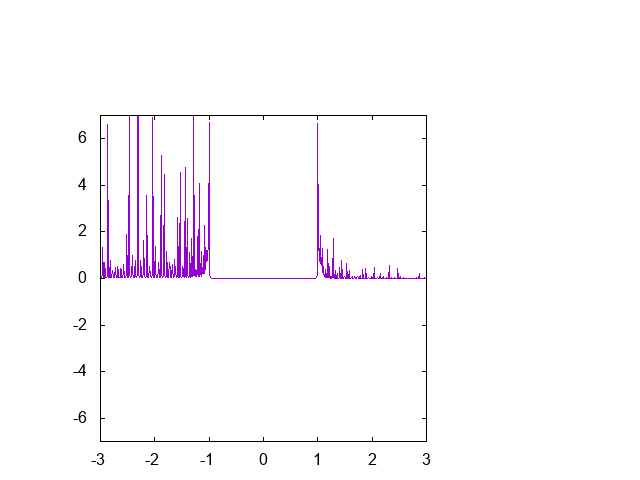
\includegraphics[scale=0.7]{../../16/KS/16-2/graph/data.png}
	\caption{状態密度}
\end{figure}
ここからエネルギーが$-1$〜$1$では状態がないことが分かる。
\subsection{2の場合}
(2)前回までに行った計算を$p_{x}-wave$に対して行う。すなわち$\hat{\Delta}(r)$を以下のようにする。
\begin{align}
\hat{\Delta}(r)=\Delta_0\dfrac{i\partial x}{k_F}\hat\sigma_1
\end{align}
このとき
\begin{align}
\hat{\sigma_1}=
\begin{pmatrix}
0 & 1\\
1 & 0
\end{pmatrix}
\end{align}
である。従って
\begin{align}
\tilde{H}&=
\begin{pmatrix}
(-\dfrac{\hbar^2}{2m}\nabla^2-\mu_F)\begin{pmatrix}
1 & 0 \\
0 & 1
\end{pmatrix} & \dfrac{\Delta_0}{k_{F}} \begin{pmatrix}
0 & i\partial x \\
i\partial x & 0
\end{pmatrix} \\
-\left(\dfrac{\Delta_0}{k_{F}}\right)^{*}
\begin{pmatrix}
0 & -i\partial x \\
-i\partial x& 0
\end{pmatrix} & (\dfrac{\hbar^2}{2m}\nabla^2+\mu_F)\begin{pmatrix}
1 & 0 \\
0 & 1
\end{pmatrix}
\end{pmatrix}
\\&=\begin{pmatrix}
\xi & 0 & 0 & \eta \\ 
0 & \xi & \eta & 0 \\ 
0 & \eta^{'} & -\xi & 0 \\ 
\eta^{'} & 0 & 0 & -\xi
\end{pmatrix} 
\end{align}
となる。ここで
\begin{align}
-\dfrac{\hbar^2}{2m}\nabla^2-\mu_F&=\xi\\
\dfrac{\Delta_0}{k_{F}}i\partial x&=\eta\\
\left(\dfrac{\Delta_0}{k_{F}}\right)^{*}i\partial x&=\eta^{'}
\end{align}
とおいた。前回との違いは$\eta$とその中に$x$の微分が入っていることなので、この項を検討していく。例えば
\begin{align}
\psi_{\downarrow}e^{-ik_{y}^{'}y}\eta\psi_{\uparrow}e^{ik_{y}^{'}y}
\end{align}
は
\begin{align}
\psi_{\downarrow}e^{-ik_{y}^{'}y}\eta\psi_{\uparrow}e^{ik_{y}^{'}y}&= \psi_{\downarrow}e^{-ik_{y}^{'}y}\dfrac{\Delta_0}{k_{F}}i\partial x\psi_{\uparrow}e^{ik_{y}^{'}y}\\
&= \psi_{\downarrow}e^{-ik_{y}^{'}y}\dfrac{\Delta_0}{k_{F}}ie^{ik_{y}^{'}y}\partial x\psi_{\uparrow}
\end{align}
となる。$\partial x\psi_{\uparrow}$を中心差分を用いて離散化していく。
\begin{align}
\dfrac{\partial}{\partial x}f(x)=\dfrac{f(x+h)-f(x-h)}{2h}
\end{align}
刻み幅$1$で$x$を$i$で書けば
\begin{align}
\dfrac{\partial}{\partial x}f(i)=\dfrac{f(x+i)-f(x-i)}{2}
\end{align}
であるから
これより$\mathcal{H}$は
\begin{align}
\mathcal{H}
=\sum_{i=1}^{L_y+1}\displaystyle\sum_{k_y}\Big[\big\{\dfrac{\hbar^2}{2m}(k_y^2+2)-\mu\big\}\psi_{i\uparrow}^{\dagger}\psi_{i\uparrow}-\Lambda\psi_{i\uparrow}^{\dagger}\psi_{i+1\uparrow}-\Lambda\psi_{i\uparrow}^{\dagger}\psi_{i-1\uparrow}+\dfrac{\Delta_0}{2k_{F}}i\psi_{i\uparrow}^{\dagger}\psi_{{i+1}\uparrow}^{\dagger}-\dfrac{\Delta_0}{2k_{F}}i\psi_{i\uparrow}^{\dagger}\psi_{{i-1}\uparrow}^{\dagger}\cdots\Big]dx
\end{align}
ここで
\begin{align}
\Lambda=\dfrac{\hbar^2}{2m}
\end{align}
とおいた。
\begin{align}
\varepsilon_{k_y}=\dfrac{\hbar^2}{2m}(k_y^2+2)-\mu\\
\dfrac{\Delta_0}{2k_{F}}i=\zeta\\
\left(\dfrac{\Delta_0}{k_{F}}\right)^{*}i=\zeta^{'}
\end{align}
とすると全体の$\mathcal{H}$は行列で書けて三つ分書くと
\begin{align}
\mathcal{H}=
\begin{bmatrix}
\psi_{1\uparrow}^\dagger \\ 
\psi_{1\downarrow}^\dagger \\ 
\psi_{1\uparrow} \\ 
\psi_{1\downarrow} \\ 
\psi_{2\uparrow}^\dagger \\ 
\psi_{2\downarrow}^\dagger \\ 
\psi_{2\uparrow} \\ 
\psi_{2\downarrow} \\ 
\psi_{3\uparrow}^\dagger \\ 
\psi_{3\downarrow}^\dagger \\ 
\psi_{3\uparrow} \\ 
\psi_{3\downarrow}
\end{bmatrix} 
^T
\begin{bmatrix}
\varepsilon_{k_y} & 0 & 0 & 0 & -\Lambda & 0 & 0 & -\zeta & 0 & 0 & 0 & 0 \\ 
0 & \varepsilon_{k_y} & 0 & 0 & 0 & -\Lambda & -\zeta & 0 & 0 & 0 & 0 & 0 \\ 
0 & 0 & -\varepsilon_{k_y} & 0 & 0 & \zeta^{*} & \Lambda & 0 & 0 & 0 & 0 & 0 \\ 
0 & 0 & 0 & -\varepsilon_{k_y} & \zeta^{*} & 0 & 0 & \Lambda & 0 & 0 & 0 & 0 \\ 
-\Lambda & 0 & 0 & \zeta & \varepsilon_{k_y} & 0 & 0 & 0 & -\Lambda & 0 & 0 & -\zeta \\ 
0 & -\Lambda & \zeta & 0 & 0 & \varepsilon_{k_y} & 0 & 0 & 0 & -\Lambda & -\zeta & 0 \\ 
0 & -\zeta^{*} & \Lambda & 0 & 0 & 0 & -\varepsilon_{k_y} & 0 & 0 & \zeta^{*} & \Lambda & 0 \\ 
-\zeta^{*} & 0 & 0 & \Lambda & 0 & 0 & 0 & -\varepsilon_{k_y} & \zeta^{*} & 0 & 0 & \Lambda \\ 
0 & 0 & 0 & 0 & -\Lambda & 0 & 0 & \zeta & \varepsilon_{k_y} & 0 & 0 & 0 \\ 
0 & 0 & 0 & 0 & 0 & -\Lambda & \zeta & 0 & 0 & \varepsilon_{k_y} & 0 & 0 \\ 
0 & 0 & 0 & 0 & 0 & -\zeta^{*} & \Lambda & 0 & 0 & -0 & -\varepsilon_{k_y} & 0 \\ 
0 & 0 & 0 & 0 & -\zeta^{*} & 0 & 0 & \Lambda & 0 & 0 & 0 & -\varepsilon_{k_y}
\end{bmatrix} 
\begin{bmatrix}
\psi_{1\uparrow} \\ 
\psi_{1\downarrow} \\ 
\psi_{1\uparrow}^\dagger \\ 
\psi_{1\downarrow}^\dagger \\ 
\psi_{2\uparrow} \\ 
\psi_{2\downarrow} \\ 
\psi_{2\uparrow}^\dagger \\ 
\psi_{2\downarrow}^\dagger \\ 
\psi_{3\uparrow} \\ 
\psi_{3\downarrow} \\ 
\psi_{3\uparrow}^\dagger \\ 
\psi_{3\downarrow}^\dagger
\end{bmatrix} 
\end{align}
となる。ここから$\mathcal{H}$を数値計算で対角化していく。
また$k_{F}$は
\begin{align}
\mu=\dfrac{\hbar^{2}k_F^{2}}{2m}
\end{align}
から求める。
先と同様に$\mathcal{H}$を数値計算で対角化していく。この時$\mu=3.5, \Lambda=1.0, \Delta=1.0$	とした。
$N=100$、$k_y$を横軸として変化させて縦軸に固有値をプロットし分散関係を描いた。結果は以下のようになった。\\
\begin{figure}[H]
	\centering
	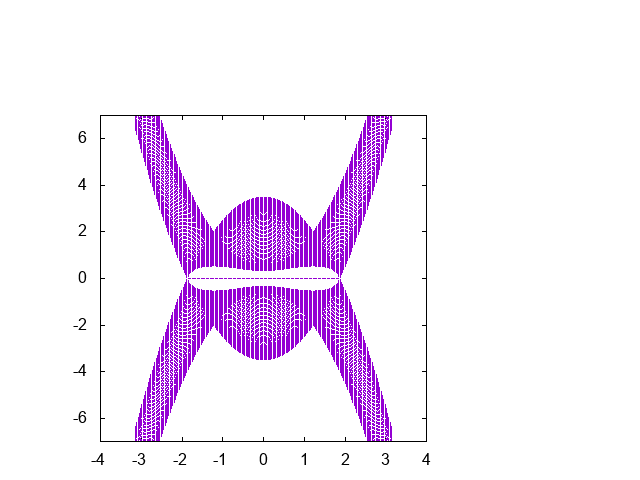
\includegraphics[scale=0.5]{../../18/KS/18-1/graph/data.png}
	\caption{分散関係}
\end{figure}
\begin{figure}[H]
	\centering
	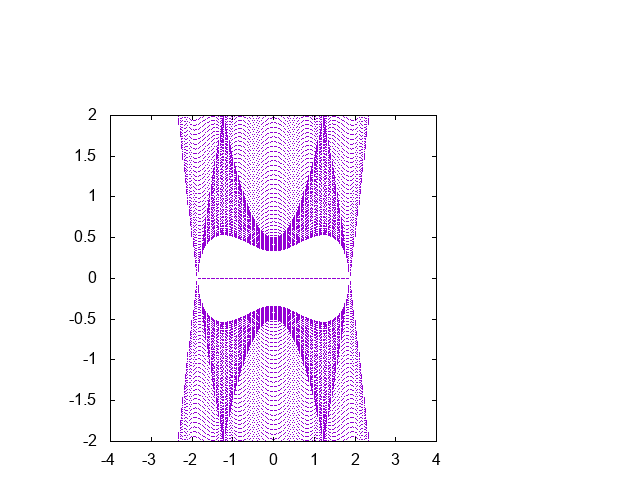
\includegraphics[scale=0.5]{../../18/KS/18-2/graph/data.png}
	\caption{分散関係:拡大}
\end{figure}
次にグリーン関数を用いて状態密度を求めた。
端には電子が存在しており、その間にエネルギー状態があるが、周りにはないことが分かる。\\
次に$E$を$-3$〜$3$で動かして$\rho$をプロットした。この時$\delta=10^{-3}$とした。
以下に結果を示す。
\begin{figure}[H]
	\centering
	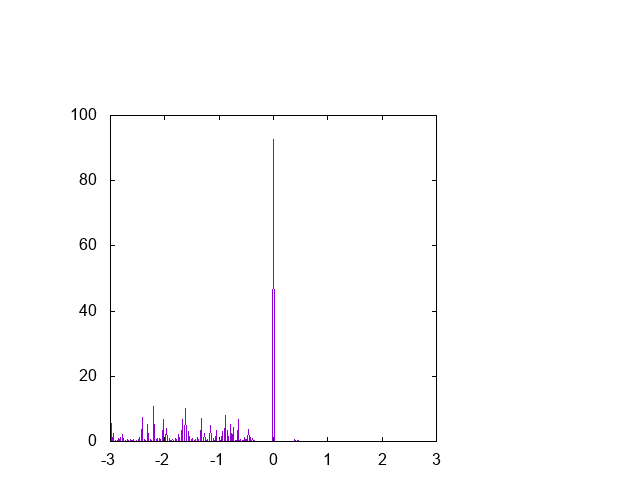
\includegraphics[scale=0.5]{../../18/KS/18-3/graph/data.png}
	\caption{表面の状態密度}
\end{figure}
ここからエネルギーが$-1$〜$1$では状態があることが分かる。これは(1)の結果とは異なる点である。\\
また内部を
\begin{align}
\rho=-\dfrac{1}{\pi}{\rm lm}(G_{201,202}+G_{202,202})			
\end{align}
で求めると
\begin{figure}[H]
	\centering
	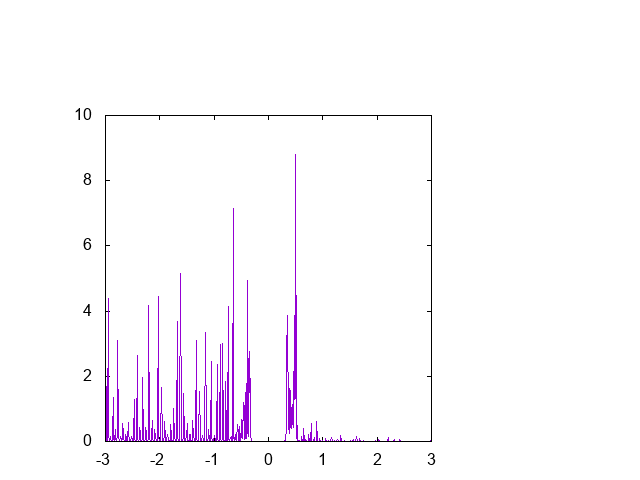
\includegraphics[scale=0.5]{../../18/KS/18-4/graph/data.png}
	\caption{内部の状態密度}
\end{figure}
のようになり、$0$付近では(1)と同じように状態がない。
\subsection{3の場合}
(2)前回までに行った計算を$p_{x}-ip_{y}wave$に対して行う。すなわち$\hat{\Delta}(r)$を以下のようにする。
\begin{align}
\hat{\Delta}(r)=\Delta_0\dfrac{\partial x+i\partial y}{k_F}\hat\sigma_1
\end{align}
このとき
\begin{align}
\hat{\sigma_1}=
\begin{pmatrix}
0 & 1\\
1 & 0
\end{pmatrix}
\end{align}
である。従って
\begin{align}
\tilde{H}&=
\begin{pmatrix}
(-\dfrac{\hbar^2}{2m}\nabla^2-\mu_F)\begin{pmatrix}
1 & 0 \\
0 & 1
\end{pmatrix} & \dfrac{\Delta_0}{k_{F}} \begin{pmatrix}
0 & \partial x+i\partial y \\
\partial x+i\partial y & 0
\end{pmatrix} \\
-\left(\dfrac{\Delta_0}{k_{F}}\right)^{*}
\begin{pmatrix}
0 & \partial x-i\partial y \\
\partial x-i\partial y& 0
\end{pmatrix} & (\dfrac{\hbar^2}{2m}\nabla^2+\mu_F)\begin{pmatrix}
1 & 0 \\
0 & 1
\end{pmatrix}
\end{pmatrix}
\\&=\begin{pmatrix}
\xi & 0 & 0 & \eta \\ 
0 & \xi & \eta & 0 \\ 
0 & \eta^{'} & -\xi & 0 \\ 
\eta^{'} & 0 & 0 & -\xi
\end{pmatrix} 
\end{align}
となる。ここで
\begin{align}
-\dfrac{\hbar^2}{2m}\nabla^2-\mu_F&=\xi\\
\dfrac{\Delta_0}{k_{F}}(\partial x+i\partial y)&=\eta\\
\left(\dfrac{\Delta_0}{k_{F}}\right)^{*}(-\partial x+i\partial y)&=\eta^{'}
\end{align}
とおいた。前回との違いは$\eta$とその中に$x$の微分が入っていることなので、この項を検討していく。例えば
\begin{align}
\psi_{\uparrow}^{\dagger}e^{-ik_{y}^{'}y}\eta\psi_{\downarrow}^{\dagger}e^{ik_{y}^{'}y}
\end{align}
は
\begin{align}
\psi_{\uparrow}^{\dagger}e^{-ik_{y}^{'}y}\eta\psi_{\downarrow}^{\dagger}e^{ik_{y}^{'}y}&= \psi_{\uparrow}^{\dagger}e^{-ik_{y}^{'}y}\dfrac{\Delta_0}{k_{F}}(\partial x+i\partial y)\psi_{\downarrow}^{\dagger}e^{ik_{y}^{'}y}\\
&=\bigl(\psi_{\uparrow}^{\dagger}e^{-ik_{y}^{'}y}e^{ik_{y}^{'}y}\dfrac{\partial}{\partial x}\psi_{\downarrow}^{\dagger}-k_{y}\psi_{\uparrow}^{\dagger}e^{-ik_{y}^{'}y}e^{ik_{y}^{'}y}\psi_{\downarrow}^{\dagger}\bigr)\dfrac{\Delta_0}{k_{F}}
\end{align}
となる。$\partial x\psi_{\uparrow}$を中心差分を用いて離散化していく。
\begin{align}
\dfrac{\partial}{\partial x}f(x)=\dfrac{f(x+h)-f(x-h)}{2h}
\end{align}
刻み幅$1$で$x$を$i$で書けば
\begin{align}
\dfrac{\partial}{\partial x}f(i)=\dfrac{f(x+i)-f(x-i)}{2}
\end{align}
であるから
これより$\mathcal{H}$の前回からの変更点は例えば
\begin{align}
\mathcal{H}
=\int\sum_{i=1}^{L_y+1}\displaystyle\sum_{k_y}\dfrac{\Delta_0}{k_{F}}\bigl\{\psi_{i\uparrow}^{\dagger}\dfrac{1}{2}\bigl(\psi_{i+1\downarrow}^{\dagger}-\psi_{i-1\downarrow}^{\dagger}\bigr)-k_{y}\psi_{i\uparrow}^{\dagger}\psi_{i\downarrow}^{\dagger}\bigr\}
\end{align}
ここで
\begin{align}
\Lambda=\dfrac{\hbar^2}{2m}\\
\varepsilon_{k_y}=\dfrac{\hbar^2}{2m}(k_y^2+2)-\mu\\
\dfrac{\Delta_0}{2k_{F}}=C\\
\end{align}
とすると全体の$\mathcal{H}$は行列で書けて三つ分書くと
\begin{align}
\mathcal{H}=
\begin{bmatrix}
\psi_{1\uparrow}^\dagger \\ 
\psi_{1\downarrow}^\dagger \\ 
\psi_{1\uparrow} \\ 
\psi_{1\downarrow} \\ 
\psi_{2\uparrow}^\dagger \\ 
\psi_{2\downarrow}^\dagger \\ 
\psi_{2\uparrow} \\ 
\psi_{2\downarrow} \\ 
\psi_{3\uparrow}^\dagger \\ 
\psi_{3\downarrow}^\dagger \\ 
\psi_{3\uparrow} \\ 
\psi_{3\downarrow}
\end{bmatrix} 
^T
\begin{bmatrix}
\varepsilon_{k_y} & 0 & 0 & -2Ck_{y} & -\Lambda & 0 & 0 & C & 0 & 0 & 0 & 0 \\ 
0 & \varepsilon_{k_y} & -2Ck_{y} & 0 & 0 & -\Lambda & C & 0 & 0 & 0 & 0 & 0 \\ 
0 & -2C^{*}k_{y} & -\varepsilon_{k_y} & 0 & 0 & -C^{*} & \Lambda & 0 & 0 & 0 & 0 & 0 \\ 
-2C^{*}k_{y} & 0 & 0 & -\varepsilon_{k_y} & -C^{*} & 0 & 0 & \Lambda & 0 & 0 & 0 & 0 \\ 
-\Lambda & 0 & 0 & -C & \varepsilon_{k_y} & 0 & 0 & -2Ck_{y} & -\Lambda & 0 & 0 & C \\ 
0 & -\Lambda & -C & 0 & 0 & \varepsilon_{k_y} & -2Ck_{y} & 0 & 0 & -\Lambda & C & 0 \\ 
0 & C^{*} & \Lambda & 0 & 0 & -2C^{*}k_{y} & -\varepsilon_{k_y} & 0 & 0 & -C^{*} & \Lambda & 0 \\ 
C^{*} & 0 & 0 & \Lambda & -2C^{*}k_{y} & 0 & 0 & -\varepsilon_{k_y} & -C^{*} & 0 & 0 & \Lambda \\ 
0 & 0 & 0 & 0 & -\Lambda & 0 & 0 & -C & \varepsilon_{k_y} & 0 & 0 & -2Ck_{y} \\ 
0 & 0 & 0 & 0 & 0 & -\Lambda & -C & 0 & 0 & \varepsilon_{k_y} & -2Ck_{y} & 0 \\ 
0 & 0 & 0 & 0 & 0 & C^{*} & \Lambda & 0 & 0 & -2C^{*}k_{y} & -\varepsilon_{k_y} & 0 \\ 
0 & 0 & 0 & 0 & C^{*} & 0 & 0 & \Lambda & -2C^{*}k_{y} & 0 & 0 & -\varepsilon_{k_y}
\end{bmatrix} 
\begin{bmatrix}
\psi_{1\uparrow} \\ 
\psi_{1\downarrow} \\ 
\psi_{1\uparrow}^\dagger \\ 
\psi_{1\downarrow}^\dagger \\ 
\psi_{2\uparrow} \\ 
\psi_{2\downarrow} \\ 
\psi_{2\uparrow}^\dagger \\ 
\psi_{2\downarrow}^\dagger \\ 
\psi_{3\uparrow} \\ 
\psi_{3\downarrow} \\ 
\psi_{3\uparrow}^\dagger \\ 
\psi_{3\downarrow}^\dagger
\end{bmatrix} 
\end{align}
となる。ここから$\mathcal{H}$を数値計算で対角化していく。
また$k_{F}$は
\begin{align}
\mu=\dfrac{\hbar^{2}k_F^{2}}{2m}
\end{align}
から求める。
先と同様に$\mathcal{H}$を数値計算で対角化していく。この時$\mu=3.5, \lambda=1.0, \Delta=1.0$	とした。
$N=100$、$k_y$を横軸として変化させて縦軸に固有値をプロットし分散関係を描いた。結果は以下のようになった。\\
\begin{figure}[H]
	\centering
	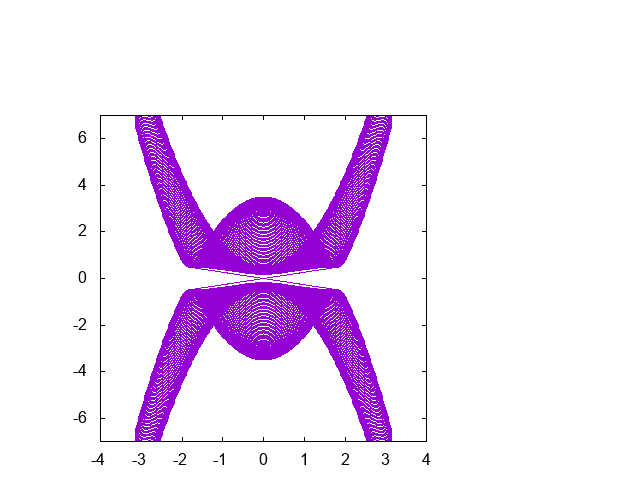
\includegraphics[scale=0.7]{../../20/KS/20-1/graph/data.png}
	\caption{分散関係}
		\label{3ek}
\end{figure}
拡大したものを示す。
\begin{figure}[H]
	\centering
	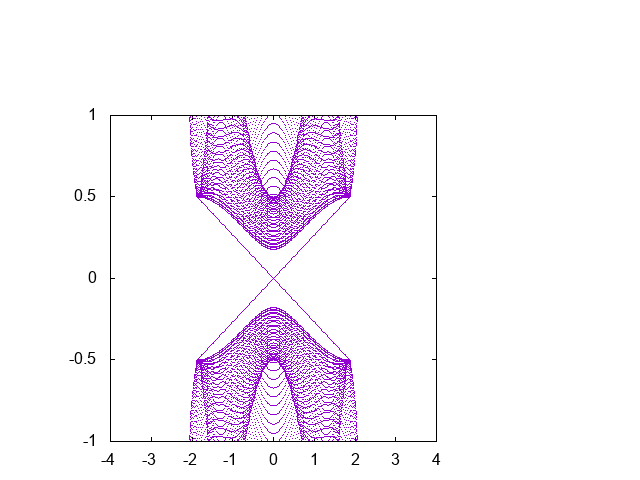
\includegraphics[scale=0.7]{../../20/KS/20-2/graph/data.png}
	\caption{分散関係の拡大}
\end{figure}
これから分かるように上と下から一本ずつ線が出て交わり、反対側に行っていることが分かる。\\
次にグリーン関数を用いて状態密度を求めた。

次に$E$を$-3$〜$3$で動かして$\rho$をプロットした。この時$\delta=10^{-3}$、$k_y=\dfrac{\pi}{4}$とした。
以下に結果を示す。
内部について
\begin{align}
\rho=-\dfrac{1}{\pi}{\rm Im}(G_{201,202}+G_{202,202})
\end{align}
で求めると
\begin{figure}[H]
	\centering
	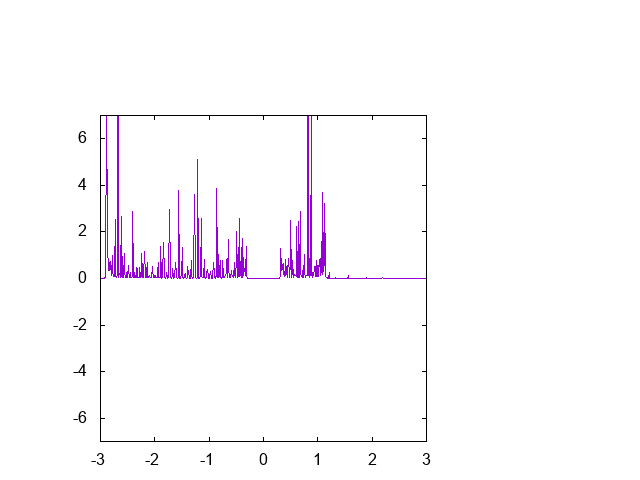
\includegraphics[scale=0.7]{../../20/KS/20-3/graph/data.png}
	\caption{内部の状態密度}
\end{figure}
のようになり、$0$付近では(1)と同じように状態がない。
また表面は以下のような結果となった。
\begin{figure}[H]
	\centering
	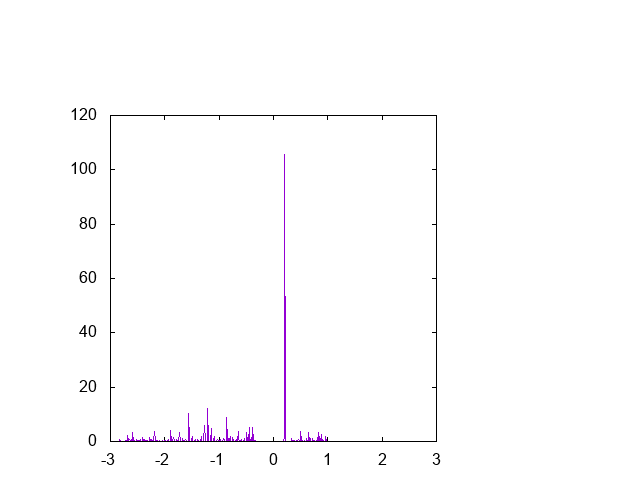
\includegraphics[scale=0.7]{../../20/KS/20-4/graph/data.png}
	\caption{表面の状態密度:左端}
\end{figure}
\begin{figure}[H]
	\centering
	\includegraphics[scale=0.7]{../../20/KS/20-5/graph/data.png}
	\caption{表面の状態密度:右端}
\end{figure}
ここからエネルギーが$-1$〜$1$では状態があることが分かる。これは(1)の結果とは異なる点である。\\
また図\ref{3ek}を見ると各波数に対して二本の状態密度が出てもいいように思える。しかし実際には一本しか観測されないのは左側と右側それぞれに対して一本ずつあり、図\ref{3ek}ではそれが合わさって見えるためだと考えられる。それぞれがどのような一本かを見るため$k_y=-\dfrac{\pi}{4}$としてプロットした。すると左側では以下のようになった。
\begin{figure}[H]
	\centering
	\includegraphics[scale=0.7]{../../20/KS/20-6/graph/data.png}
	\caption{表面の状態密度:左端}
\end{figure}
すなわち、左側の状態では左下から右上に直線的に伸びていることが分かった。
\end{document}